%%%%%%%% ICML 2026 EXAMPLE LATEX SUBMISSION FILE %%%%%%%%%%%%%%%%%

\documentclass{article}

% Recommended, but optional, packages for figures and better typesetting:
\usepackage{microtype}
\usepackage{graphicx}
\usepackage{subcaption}
\usepackage{booktabs} % for professional tables

\usepackage{bm}

\newcommand{\e}{{\mathrm{e}}}
\renewcommand{\i}{{\mathrm{i}}}
\newcommand{\dd}{{\mathrm{d}}}

% hyperref makes hyperlinks in the resulting PDF.
% If your build breaks (sometimes temporarily if a hyperlink spans a page)
% please comment out the following usepackage line and replace
% \usepackage{icml2026} with \usepackage[nohyperref]{icml2026} above.
\usepackage{hyperref}


% Attempt to make hyperref and algorithmic work together better:
\newcommand{\theHalgorithm}{\arabic{algorithm}}

% Use the following line for the initial blind version submitted for review:
\usepackage{icml2026}

% For preprint, use
% \usepackage[preprint]{icml2026}

% If accepted, instead use the following line for the camera-ready submission:
% \usepackage[accepted]{icml2026}

\usepackage{amsmath}
\usepackage{amssymb}
\usepackage{mathtools}
\usepackage{amsthm}


% if you use cleveref..
\usepackage[capitalize,noabbrev]{cleveref}

%%%%%%%%%%%%%%%%%%%%%%%%%%%%%%%%
% THEOREMS
%%%%%%%%%%%%%%%%%%%%%%%%%%%%%%%%
\theoremstyle{plain}
\newtheorem{theorem}{Theorem}[section]
\newtheorem{proposition}[theorem]{Proposition}
\newtheorem{lemma}[theorem]{Lemma}
\newtheorem{corollary}[theorem]{Corollary}
\theoremstyle{definition}
\newtheorem{definition}[theorem]{Definition}
\newtheorem{assumption}[theorem]{Assumption}
\theoremstyle{remark}
\newtheorem{remark}[theorem]{Remark}

% Todonotes is useful during development; simply uncomment the next line
%    and comment out the line below the next line to turn off comments
%\usepackage[disable,textsize=tiny]{todonotes}
\usepackage[textsize=tiny]{todonotes}

% The \icmltitle you define below is probably too long as a header.
% Therefore, a short form for the running title is supplied here:
\icmltitlerunning{Geometric Entropy and Retrieval Phase Transitions in Continuous DAM}

\begin{document}

\twocolumn[
  \icmltitle{Geometric Entropy and Retrieval Phase Transitions\\
  in Continuous Dense Associative Memory}

  % It is OKAY to include author information, even for blind submissions: the
  % style file will automatically remove it for you unless you've provided
  % the [accepted] option to the icml2026 package.

  % List of affiliations: The first argument should be a (short) identifier you
  % will use later to specify author affiliations Academic affiliations
  % should list Department, University, City, Region, Country Industry
  % affiliations should list Company, City, Region, Country

  % You can specify symbols, otherwise they are numbered in order. Ideally, you
  % should not use this facility. Affiliations will be numbered in order of
  % appearance and this is the preferred way.
  \icmlsetsymbol{equal}{*}

  \begin{icmlauthorlist}
    \icmlauthor{Firstname1 Lastname1}{equal,yyy}
    \icmlauthor{Firstname2 Lastname2}{equal,yyy,comp}
    \icmlauthor{Firstname3 Lastname3}{comp}
    \icmlauthor{Firstname4 Lastname4}{sch}
    \icmlauthor{Firstname5 Lastname5}{yyy}
    \icmlauthor{Firstname6 Lastname6}{sch,yyy,comp}
    \icmlauthor{Firstname7 Lastname7}{comp}
    %\icmlauthor{}{sch}
    \icmlauthor{Firstname8 Lastname8}{sch}
    \icmlauthor{Firstname8 Lastname8}{yyy,comp}
    %\icmlauthor{}{sch}
    %\icmlauthor{}{sch}
  \end{icmlauthorlist}

  \icmlaffiliation{yyy}{Department of XXX, University of YYY, Location, Country}
  \icmlaffiliation{comp}{Company Name, Location, Country}
  \icmlaffiliation{sch}{School of ZZZ, Institute of WWW, Location, Country}

  \icmlcorrespondingauthor{Firstname1 Lastname1}{first1.last1@xxx.edu}
  \icmlcorrespondingauthor{Firstname2 Lastname2}{first2.last2@www.uk}

  % You may provide any keywords that you find helpful for describing your
  % paper; these are used to populate the "keywords" metadata in the PDF but
  % will not be shown in the document
  \icmlkeywords{Machine Learning, ICML}

  \vskip 0.3in
]

% this must go after the closing bracket ] following \twocolumn[ ...

% This command actually creates the footnote in the first column listing the
% affiliations and the copyright notice. The command takes one argument, which
% is text to display at the start of the footnote. The \icmlEqualContribution
% command is standard text for equal contribution. Remove it (just {}) if you
% do not need this facility.

% Use ONE of the following lines. DO NOT remove the command.
% If you have no special notice, KEEP empty braces:
\printAffiliationsAndNotice{}  % no special notice (required even if empty)
% Or, if applicable, use the standard equal contribution text:
% \printAffiliationsAndNotice{\icmlEqualContribution}

\begin{abstract}
We derive thermodynamic phase boundaries for Dense Associative Memory networks with exponential capacity $p = e^{\alpha N}$, comparing Gaussian (LSE) and Epanechnikov (LSR) kernels. For continuous neurons on an $N$-sphere, the geometric entropy depends solely on the spherical geometry, not the kernel. Sufficiently sharp kernels achieve maximum theoretical capacity $\alpha = 0.5$ at zero temperature; below this threshold, a critical line separates retrieval from a spin-glass phase. Kernel sharpness introduces a trade-off between energetic stability and entropic cost: while LSR provides deeper energy minima, it exhibits a smaller retrieval region than LSE at finite temperature because enforcing higher alignment incurs a geometric entropy penalty that outweighs the energetic gain. The kernels also differ qualitatively in their thermal limits: LSR possesses a finite maximum retrieval temperature, whereas LSE permits retrieval at arbitrarily high temperatures for sufficiently low loads.
\end{abstract}

\section{Introduction}

Dense Associative Memory (DAM) networks extend classical Hopfield models by replacing pairwise interactions with highly nonlinear energy functions, substantially improving storage capacity and robustness. When defined over continuous states constrained to an $N$-dimensional sphere, DAMs can store an exponential number of patterns ($p = \exp(\alpha N)$) with perfect recall in the zero-temperature limit \citep{demircigil2017model,ramsauer2021hopfield,lucibello2024exponential}. These models have garnered renewed interest due to their formal equivalence to softmax attention mechanisms in Transformers, where energy-based updates closely mirror attention-driven memory retrieval \citep{ramsauer2021hopfield}. However, existing theoretical results largely describe behavior at zero temperature, leaving open how retrieval stability persists under noise and thermal fluctuations.

Recent work has revisited associative memory from a thermodynamic perspective. Building on the classical theory of retrieval-to-spin-glass transitions in Hopfield networks \citep{amit1987statistical}, \citet{rooke2026stochastic} introduced a stochastic thermodynamics framework for DAMs, quantifying entropy production during retrieval and highlighting trade-offs between energetic cost and recall performance. In parallel, \citet{lucibello2024exponential} analyzed retrieval stability in DAMs with exponential capacity, emphasizing entropic penalties that arise in high-dimensional settings. These developments motivate a finite-temperature theory of retrieval in continuous, high-capacity associative memory systems.

Our work is most closely related to \citet{lucibello2024exponential}. While both studies address exponential memory load and thermodynamic limits, \citet{lucibello2024exponential} primarily focus on zero-temperature or energy-dominated regimes. In contrast, we derive explicit finite-temperature phase boundaries for continuous DAMs on the $N$-sphere and show that retrieval stability is governed by a competition between kernel-dependent energy and a kernel-independent \emph{geometric entropy} term induced solely by the spherical constraint. This separation enables a principled comparison of different kernels and reveals qualitative differences in thermal robustness, including a finite maximal retrieval temperature for compactly supported kernels.

We analytically characterize the thermodynamic retrieval phase of continuous DAMs under finite temperature and exponential memory load. Specifically, we derive the phase boundary $\alpha_c(T)$ in the $(\alpha,T)$ plane separating retrieval from disordered behavior. We study DAMs on the $N$-sphere with two kernel-based energy functions: the Gaussian log-sum-exp (LSE) and the compactly supported log-sum-ReLU (LSR) \citep{hoover2025dense}. Although both achieve exponential capacity as $T \to 0$, they differ in how kernel sharpness mediates robustness to thermal noise.

In the high-dimensional regime, increasing the number of stored patterns reduces their typical angular separation, and sharper kernels impose a stronger entropic cost to maintain high alignment with a target pattern. As a result, LSR exhibits a finite critical temperature beyond which retrieval becomes thermodynamically unstable, whereas LSE can remain stable at arbitrarily high temperatures under sufficiently low load.

Our contributions are:
\begin{enumerate}
    \item Analytical characterization of the finite-temperature retrieval transition in continuous DAMs with exponential memory load.
    \item Identification of a kernel-independent geometric entropy term for retrieval on the $N$-sphere and analysis of its competition with kernel-dependent energetic stabilization.
    \item Derivation of explicit analytical phase boundaries for LSE and LSR kernels, revealing a finite maximal retrieval temperature for LSR and unbounded thermal stability for LSE at low load.
\end{enumerate}

These results extend thermodynamic analyses of high-capacity associative memory to continuous spherical DAMs at finite temperature, clarifying which aspects of retrieval robustness are universal consequences of geometry and which depend on the associative kernel.






\section{Dense Associative Memory networks}

In the study of Dense AM (Associative Memory), two types of Hamiltonians that define the internal energy of the system are distinguished. The first type is $k$-polynomial~\cite{krotov2016dense}, 
\begin{equation}
    H_k(\bm{x}) = - \frac{1}{N^{k-1}} \sum\limits_{\mu=1}^{M} (\bm{x} \cdot \bm{\xi}^\mu)^k\,,
    \label{eq:H_k}
\end{equation}
a special case of which is the classical Hopfield network \cite{Hopfield1982} when $k=2$. 
The vectors $\bm{x}$ and $\bm{\xi}^\mu$ belong to the same space and define, respectively, the current state of the system and the stored patterns (memories, $\mu=1\dots M$). They can either be simply elements of the binary neuron space $\{-1,+1\}^N$, or be continuous, for example, bounded on each coordinate by the interval $[-1, 1]$. This type is characterized by polynomial capacity $M_{\rm max} = \alpha N^{k-1}$~\cite{krotov2016dense}. In particular, for the Hopfield network with spins, the well known result is $M_{\rm max} \approx 0.14N$.

The second type of Hamiltonians is the exponential interaction type. The connection to polynomial interactions arises in the limiting case $k \to \infty$, where polynomial terms give way to exponential ones. This modification yields a maximum capacity of $M_{\rm max} \approx \exp(\alpha N)$, with $\alpha \approx 0.35$ for binary spin data~\cite{demircigil2017model}.

\citet{ramsauer2021hopfield} extended these exponential capacity results to continuous states using the Log-Sum-Exp (LSE) energy function, 
\begin{equation}
    H_{\rm LSE}(\bm{x}) \propto -\ln \left( \sum_{\mu=1}^M \exp(\beta_{\rm net} \, \bm{x} \cdot \bm{\xi}^\mu) \right) \,,
    \label{eq:lse_energy}
\end{equation}
establishing a direct link to modern Deep Learning.
The update rule minimizing this energy is mathematically equivalent to the self-attention mechanism in Transformers, where stored patterns serve as Keys and the state vector as a Query. To satisfy the geometric requirements of continuous attention and maintain consistency with LayerNorm, vector magnitudes must be constrained. Hereafter, we assume continuous real-valued coordinates with vectors normalized according to $\sum_{i=1}^{N} x_i^2 = N$ (the $N$-sphere model). Under this spherical constraint, the continuous model achieves a higher capacity coefficient than the binary case: \citet{ramsauer2021hopfield} proved that $M_{\rm max} \propto \exp(\alpha N)$ with $\alpha = 0.5$.

While the dot product formulation is central to the Transformer interpretation, \citet{krotov2021large} introduced an alternative formulation based on Euclidean distance $d^2(\bm{x}, \bm{\xi}^\mu) = \|\bm{x}-\bm{\xi}^\mu\|^2$ to model prototype-based learning. This yields a kernel-based energy function:
\begin{equation}
    H_{\rm LSE}(\bm{x}) = -\frac{1}{\beta_{\rm net}} \ln p(\bm{x}, \bm{\xi}^\mu) \,.
    \label{eq:H_lse}
\end{equation}
with 
\begin{equation}
    p(\bm{x}, \bm{\xi}^\mu) \equiv \sum_{\mu=1}^M \exp\left[ - \frac{\beta_{\rm net}}{2} d^2(\bm{x}, \bm{\xi}^\mu) \right] \,.
    \label{eq:dens}
\end{equation}
This form admits a statistical interpretation: the energy corresponds to the negative log-likelihood of a Kernel Density Estimate (KDE) of the memory distribution with a Gaussian kernel~\cite{hoover2025dense}. Under the $N$-sphere constraint, however, these two formulations are  equivalent, since 
\begin{equation}
    d^2(\bm{x}, \bm{\xi}^\mu) = \|\bm{x}\|^2 + \|\bm{\xi}^\mu\|^2 - 2\bm{x} \cdot \bm{\xi}^\mu = 2N - 2\bm{x} \cdot \bm{\xi}^\mu \,.
    \label{eq:edist}
\end{equation}

The parameter $\beta_{\rm net}$, termed the {\it inverse variance}, has nothing to do with the outer thermal bath. Rather, it defines the shape of the energy landscape by controlling the sharpness of the kernel related to its effective width $\sigma$ by:
\begin{equation}
    \sigma^2 \equiv \beta_{\rm net}^{-1} \,.
\end{equation}

Recently, \citet{hoover2025dense} proposed the log-sum-ReLU (LSR) energy function, inspired by optimal kernel density estimation using the Epanechnikov kernel. This formulation achieves exact memory retrieval with exponential capacity without relying on exponential kernels:
\begin{equation}
    H_{\rm LSR}(\bm{x}) = -\frac{1}{\beta_{\rm net}} \ln \left( \sum_{\mu=1}^M \max\left[\epsilon,  1 - \frac{d^2(\bm{x},\bm{\xi}^\mu)}{2\sigma^2} \right] \right) \,,
    \label{eq:H_lsr}
\end{equation}
where $\epsilon > 0$ is a small constant introduced to prevent singularities in the logarithm.

Memory retrieval occurs when patterns are sufficiently separated from one another, while the initial network state corresponding to a corrupted pattern lies within the basin of attraction of the target pattern. The quantity characterizing this proximity is called \textit{alignment}:
\begin{equation}
    \phi^\mu(\bm{x}) = \frac{1}{N} \bm{x} \cdot \bm{\xi}^\mu\,,
    \label{eq:alignment}
\end{equation}
taking $\phi^\mu(\bm{x}) \approx 1$ when the vectors are close, and close to zero otherwise. The Euclidean distance (\ref{eq:edist}) is then expressed as $d^2(\bm{x}, \bm{\xi}^\mu) =2N [1- \phi^\mu(\bm{x}) ]$, and 
LSE/LSR Hamiltonians near a pattern $\xi$ are $H\approx N(1-\phi)$.

When the width $\sigma$ is small, the minima are well separated. Because LSE kernels are everywhere nonzero, gradient descent converges to one of the local minima regardless of initialization. For LSR, successful retrieval requires the initial state to lie within the basin of attraction of a stored pattern. As $\sigma$ increases, the two models exhibit distinct behaviors. In the LSE case, nearby patterns simply merge into a single basin. In contrast, LSR admits a narrow intermediate regime in which spurious local minima can emerge between patterns. Further increasing $\sigma$ eventually causes basins to merge, recovering the same behavior as in the LSE case~\cite{hoover2025dense}.

\section{Statistical Mechanics of Retrieval}

Thermal Dense AM is characterized by two distinct sources of randomness. The first, common to standard Dense AM, arises from the random distribution of patterns across the state space (quenched disorder), which, together with the inverse variance $\beta_{\rm net}$, determines a particular realization of the energy landscape. The second is a stochastic process originating from the interaction of the network with an environment, or thermal bath, at temperature $T$; the system is assumed to be in thermodynamic equilibrium with this bath. To analyze phase transitions in Dense AM within the statistical mechanics framework, one must pass from a microscopic to a macroscopic description, take the thermodynamic limit $N \to \infty$, and account for the random nature of the patterns $\xi^\mu$ by performing disorder averaging in the final expressions.

\subsection{The Macroscopic Framework and the Replica Method}

The Hamiltonians (\ref{eq:H_k}, \ref{eq:H_lse}, \ref{eq:H_lsr}) are readily expressed in terms of the alignments, e.g.:
\begin{multline}
    H_{\rm LSE}(\bm{x}) \equiv U_{\rm LSE}(\phi^1, \dots, \phi^M) = \\ -\frac{1}{\beta_{\rm net}} \ln \left[ \sum_{\mu=1}^M \exp\left( -\frac{N(1 - \phi^\mu)}{\sigma^2} \right) \right]\,.
\end{multline}

The thermodynamic behavior is governed by the partition function $Z$, which uses the thermodynamic $\beta = 1/T$:
\begin{equation}
    Z = \!\int\!\dd \bm{x} \exp\left( -\beta H(\bm{x}) \right) = \!\int\! \dd \bm{x} \left[ p(\bm{x}, \bm{\xi}^\mu) \right]^{\beta/\beta_{\rm net}}\!.
    \label{eq:partition}
\end{equation}

To evaluate the universal behavior of the network, we must calculate the average free energy density over the quenched disorder of the memories, $\langle f \rangle = -(N\beta)^{-1} \langle \ln Z \rangle$. The latter quantity can be evaluated using the replica identity~\cite{sk75}:
\begin{equation}
    \langle \ln Z \rangle = \lim_{n \to 0} \frac{\langle Z^n \rangle - 1}{n}
    \label{eq:limit}
\end{equation}
Derivation of $\langle Z^n \rangle$ requires shifting from the microscopic integral over $N$ neurons to a macroscopic description using alignments and averaging over overlaps (see Appendix A for details). The final expression can be written in a standard form:
\begin{equation}
    \langle f \rangle = -\frac{1}{N\beta} \langle \ln Z \rangle 
    \approx  u(\phi) - T s(\phi, q)\,,
\end{equation}
where  $s(\phi, q)$ is the entropy density, and $u(\phi)$ is the internal energy density of a single memory basin. For LSE and LSR kernels, it is given by (see Appendix A and B):
\begin{equation}
    u_{\rm LSE} = 1-\phi\,,
\end{equation}
and 
\begin{equation}
    u_{\rm LSR} = -\hat\beta^{-1}_{\rm net} \ln \Big(1 - \hat\beta_{\rm net} (1-\phi) \Big)\,.
\end{equation}

\subsection{Geometric Entropy on the $N$-sphere}

To derive the entropy, we should find the volume of the configuration space $\Omega$ that satisfies specific alignment constraints $\bm{\phi} = (\phi^1, \dots, \phi^M)^T$. We decompose the vector $\bm{x}$ into two orthogonal components: the projection $\bm{x}_{\parallel}$ onto the subspace spanned by the $M$ memories, and the component $\bm{x}_{\perp}$ in the remaining $N-M$ dimensions. It is assumed here that $M<N$, however for the phase transition study we need $M=1$ case only.

Assuming the memories are linearly independent, the squared norm of the parallel component is given by the quadratic form:
\begin{equation}
    \|\mathbf{x}_{\parallel}\|^2 = N \bm{\phi}^T G^{-1} \bm{\phi}
\end{equation}
where $G_{\mu\nu} = \frac{1}{N} \bm{\xi}^\mu \cdot \bm{\xi}^\nu$ is the Gram matrix. Because the total norm is fixed to $N$, the radius of the fluctuations in the perpendicular dimensions is:
\begin{equation}
    \|\mathbf{x}_{\perp}\|^2 = N \left( 1 - \bm{\phi}^T G^{-1} \bm{\phi} \right).
\end{equation}
The volume $\Omega(\bm{\phi})$ is proportional to the surface area of a sphere in the remaining $N-M$ dimensions with radius $R = [\|\mathbf{x}_{\perp}\|^2]^{1/2}$. The surface area of an $N-M$-sphere of radius $R$ is $A_{N-M}(R) \propto R^{N-M-1}$, therefore:
\begin{equation}
    \Omega(\bm{\phi}) \propto \left[ N \left( 1 - \bm{\phi}^T G^{-1} \bm{\phi} \right) \right]^{(N-M-1)/2}\,.
\end{equation}
In the large $N$ limit, the entropy $S = \ln \Omega$ (discarding $\phi$-independent constants) is:
\begin{equation}
    S(\bm{\phi}) = \frac{N-p}{2} \ln \left( 1 - \bm{\phi}^T G^{-1} \bm{\phi} \right).
\end{equation}

If memories are weakly correlated,  
\begin{equation}
    G_{\mu\nu} = \frac{1}{N} \bm{\xi}^\mu \cdot \bm{\xi}^\nu = I + \epsilon_{\mu\nu}\,,
\end{equation}
where $\epsilon_{\mu\nu}$ contains small off-diagonal correlations, and
in the first-order one can have:
\begin{equation}
    \bm{\phi}^T G^{-1} \bm{\phi} \approx \sum_{\mu=1}^{M} (\phi^\mu)^2 - \sum_{\mu \neq \nu} \epsilon_{\mu\nu} \phi^\mu \phi^\nu \le 1\,.
    \label{eq:gram1}
\end{equation}

For a single memory in the limit of $N\to \infty$, the entropy density is:
\begin{equation}
    s(\phi) \equiv \frac{S(\phi)}N = \frac12 \ln ( 1 - \phi^2 )
\end{equation}

The expression above is obtained for the alignment of a single microstate. In the thermal setting, the Replica Symmetry ansatz,  we assume that the system is in a thermal cloud centered at a point that has alignment $\phi$ with the target pattern $\bm{\xi}$. Thus, we change it to the alignment of the \textit{average} state.  We introduce the self-overlap parameter $q$:
\begin{equation}
    q = \frac{1}{N} \langle \bm{x} \rangle \cdot \langle \bm{x} \rangle\,,
\end{equation}
that measures the \textit{tightness} of this cloud on the $N$-sphere. As $T \to 0$, the cloud collapses to a point and $q \to 1$. As $T \to \infty$, the cloud expands to cover the sphere and $q \to 0$. The variance of thermal fluctuations is $1-q$.

The geometric entropy should be generalized to take into account the cloud tightness $q$~\cite{gardner1988space}:
\begin{equation}
    s(\phi, q) = \frac{1}{2} \ln(1-q) + \frac{q - \phi^2}{2(1-q)}.
\end{equation}

\subsection{Crosstalk and the Melted Branch}

In classical associative memory models with linear load $M = \alpha N$, interference between stored patterns manifests as local Gaussian noise \cite{amit1987statistical}. This crosstalk is captured by a term $a(M, q)$ in the total free energy density:
\begin{equation}
    f(\phi, q) = u(\phi) - T s(\phi, q) + a(M, q).
    \label{eq:total_free_energy}
\end{equation}
For the quadratic Hopfield model, $a_{\text{AGS}}(\alpha, q) = -\frac{\alpha}{2\beta} \ln [1 - \beta(1 - q)]$ acts as a repulsive potential that destabilizes retrieval when the load $\alpha$ becomes too high.

However, for exponential capacity $M = e^{\alpha N}$, the local Gaussian approximation fails. The retrieval branch must compete with an exponentially large number of spurious states, a landscape best described by the Random Energy Model (REM) \cite{derrida1980random}. Because $M$ is exponential in $N$, random configurations will almost always find accidental alignments with some pattern, creating a ``noise floor'' that competes with the intended retrieval state.

In this regime, the system exhibits two competing thermodynamic branches:
\begin{itemize}
    \item \textbf{Retrieval branch}: The system is localized near a target pattern ($\phi \approx 1$). The sharply peaked kernels suppress contributions from non-target patterns, so $a(M,q) \to 0$ and the free energy is $f_{\rm ret}(\phi, q) = u(\phi) - T s(\phi, q)$.
    \item \textbf{Melted branch}: A disordered state ($\phi = 0$) where the energy $u_{\rm melt}$ is determined by the collective interference of the $M$ patterns via REM statistics.
\end{itemize}

We define \textbf{successful retrieval} as the existence of a thermodynamically dominant retrieval state with non-zero overlap $\phi$ with a stored pattern, corresponding to a local minimum of the free energy that remains stable against the disordered (melted) phase.
Because the LSE and LSR energy wells are extremely sharp, the transition from retrieval to the disordered state is a first-order jump (melting). The retrieval phase is thermodynamically stable if and only if:
\begin{equation}
    \min_{\phi, q} \left[ u(\phi) - T s(\phi, q) \right] \leq u_{\rm melt}.
\end{equation}
As $T$ increases, the geometric entropy $s$ grows, pushing the retrieval free energy up. Simultaneously, as the load $\alpha$ increases, the noise floor $u_{\rm melt}$ drops. The transition occurs at the critical temperature $T_c$ where these two values cross, and the system instantaneously ``boils'' out of the retrieval well. We now derive $u_{\rm melt}$ for each kernel.


\subsubsection{LSE Noise Floor $u_{\rm melt}$}

To derive the energy of this melted branch, we evaluate the partition function of the $M$ non-retrieved patterns. For random state  uncorrelated with a memory, the macroscopic alignments $\phi$ follow a Gaussian distribution $P(\phi) \sim \exp(-N\phi^2/2)$. The density of patterns at a given alignment $\phi$ is $n(\phi) = M P(\phi) = \exp(N[\alpha - \phi^2/2])$. Condition $n(\phi) \sim 1$ gives the maximum spurious alignment value 
\begin{equation}
    \phi_{\rm max} = [2\alpha]^{1/2}\,.
    \label{eq:max_spur}
\end{equation}

For the LSE kernel, the density of the noise branch is determined by the sum:
\begin{multline}
    p_{\rm noise} = \sum_{\mu=1}^{M} \exp\left( -\beta_{\rm net} N (1 - \phi^\mu) \right) \approx \\
    \int \dd\phi \exp\left( N \left[ \alpha - \beta_{\rm net}(1 - \phi) - \frac{\phi^2}{2} \right] \right),
\end{multline}
where $\beta_{\rm net}$ characterizes the kernel sharpness. The internal energy density $u_{\rm melt} = - [{N\beta_{\rm net}}]^{-1} \ln p_{\rm noise}$ is dominated by the maximum of the exponent 
\begin{equation}
    g(\phi) = \alpha - \beta_{\rm net} u(\phi) - \phi^2/2\,.
    \label{eq:g_phi}
\end{equation}
The saddle point is found at $\phi^* = \beta_{\rm net}$, but this is constrained by (\ref{eq:max_spur}). This leads to two distinct thermodynamic regimes for the crosstalk:

\begin{enumerate}
    \item \textbf{Spin-Glass Regime} ($\beta_{\rm net} > \sqrt{2\alpha}$): 
    When the kernel is sufficiently sharp, the saddle point $\phi^*$ lies beyond the available patterns. The sum is dominated by the maximum spurious alignment, $\phi_{\rm max}$:
    \begin{equation}
        u_{\rm melt} = 1 - \sqrt{2\alpha}.
    \end{equation}
    In this regime, the system is frozen into the most favorable spurious alignments (spin-glass).
    
    \item \textbf{Paramagnetic Regime} ($\beta_{\rm net} < \sqrt{2\alpha}$): 
    When the kernel is blunt, the saddle point $\phi^* = \beta_{\rm net}$ is reachable, and $u_{\rm melt}$ is determined by the saddle point:
    \begin{equation}
        u_{\rm melt} = 1 - \frac{\alpha}{\beta_{\rm net}} - \frac{\beta_{\rm net}}{2}.
    \end{equation}
    Here, the noise floor is formed as a collective result of many moderate alignments (paramagnetic).
\end{enumerate}

In the subsequent phase transition analysis, we will use these REM-derived noise floors to determine the critical temperature $T_c$ and load $\alpha_c$ where the retrieval branch ($\phi > 0$) ceases to be the global minimum of the free energy.

\subsubsection{LSR Noise Floor $u_{\rm melt}$}

In the case of the Epanechnikov (LSR) kernel, the derivation of the noise floor must account for the kernel's finite support. A random pattern $\mu$ contributes to the collective noise only if its alignment falls within the support region $\phi^\mu > 1 - 1/\hat\beta_{\rm net}$, where $\hat\beta_{\rm net}$ is the rescaled network sharpness.

Following the same Random Energy Model (REM) logic as the LSE case, the maximum spurious alignment available among the $M$ patterns is $\phi_{\rm max} = [2\alpha]^{1/2}$. However, for the LSR kernel, a ``melted'' branch only exists if $\phi_{\rm max}$ exceeds the support boundary. This defines a support threshold:
\begin{equation}
    \alpha_{\rm th} = \frac{1}{2} (1 - 1/\hat\beta_{\rm net})^2 .
    \label{eq:alpha_th}
\end{equation}
If $\alpha < \alpha_{\rm th}$, the expected number of random patterns within the support of any state is effectively zero, and a disordered melted branch cannot form. For $\alpha > \alpha_{\rm th}$, the noise floor is determined by the LSR energy density:
\begin{equation}
    u_{\rm LSR}(\phi) = -\hat\beta_{\rm net}^{-1} \ln ( 1 - \hat\beta_{\rm net}(1 - \phi) )\,.
\end{equation}
Similarly to LSE, one can obtain from (\ref{eq:g_phi}) the saddle point $\phi^*$ via the equation:
\begin{equation}
    \beta_{\rm net} = f(\phi^*) = \frac{\phi^*}{1 + \phi^* - (\phi^*)^2}\,.
\end{equation}

This leads to the following regimes:
\begin{enumerate}
    \item \textbf{Spin-Glass Regime} ($\beta_{\rm net} > f(\phi_{\rm max})$): 
    The integral is dominated by the patterns at the edge of the distribution, $\phi_{\rm max}$. The noise floor energy is given by the value of the logarithmic well at the maximum spurious alignment:
    \begin{equation}
        u_{\rm melt} = -\frac{1}{\beta_{\rm net}} \ln \left( 1 - \beta_{\rm net} (1 - \sqrt{2\alpha}) \right).
    \end{equation}
    In this regime, the system is trapped by the best spurious alignments among the exponentially many patterns. Unlike the LSE case, this energy diverges as the load approaches the theoretical limit where $\sqrt{2\alpha} \to 1 - 1/\hat\beta_{\rm net}$.
    
    \item \textbf{Paramagnetic Regime} ($\beta_{\rm net} < f(\phi_{\rm max})$): 
    The collective noise floor is determined by the reachable saddle point $\phi^*$. 
    \begin{equation}
        u_{\rm melt} = u(\phi^*)\,.
    \end{equation}
    
\end{enumerate}


The crucial difference for LSR is that $u_{\rm melt}$ diverges as the temperature increases or the load decreases toward the support boundary. This reflects the "logarithmic well" mentioned in the abstract, which forces the retrieval phase to "boil" into a disordered state at a finite maximum temperature $T_{\rm max}$, a behavior qualitatively different from the unbounded thermal robustness of the LSE kernel.



\section{Experiments. Equilibrium Analysis and Critical Lines}

Having established the free energy framework, we now derive the equilibrium states and critical phase boundaries for both kernels. The key insight is that despite sharing the same geometric entropy, the different energy functions lead to qualitatively distinct phase diagrams.

\subsection{LSE Equilibrium}

For the Gaussian (LSE) kernel with energy density $u_{\rm LSE}(\phi) = 1 - \phi$, the retrieval free energy is:
\begin{equation}
    f_{\rm ret}(\phi, q) = (1 - \phi) - T \left[ \frac{1}{2}\ln(1-q) + \frac{q - \phi^2}{2(1-q)} \right].
\end{equation}
Minimizing over $q$ and $\phi$ yields two equilibrium conditions. The first, $\partial f/\partial q = 0$, gives:
\begin{equation}
    q = \phi^2,
    \label{eq:q_constraint}
\end{equation}
meaning the thermal cloud tightness is entirely determined by the alignment. The second, $\partial f/\partial \phi = 0$, gives:
\begin{equation}
    -1 + \frac{T\phi}{1-\phi^2} = 0 \quad \Rightarrow \quad \phi^2 + T\phi - 1 = 0.
\end{equation}
The physical solution (with $\phi \to 1$ as $T \to 0$) is:
\begin{equation}
    \phi_{\rm LSE}(T) = \frac{-T + \sqrt{T^2 + 4}}{2}
    \label{eq:phi_lse}
\end{equation}
Substituting the equilibrium values into the free energy:
\begin{equation}
    f_{\rm ret}^{\rm LSE}(T) = (1 - \phi) - \frac{T}{2}\ln(1 - \phi^2).
    \label{eq:f_lse}
\end{equation}
At $T = 0$, $\phi = 1$ and $f_{\rm ret} = 0$. As $T \to \infty$, $\phi \to 0$ and $f_{\rm ret} \to 1$.

\paragraph{Critical Line.} The phase boundary occurs where $f_{\rm ret}(T) = u_{\rm melt}(\alpha)$. In the spin-glass regime ($\beta_{\rm net} > \sqrt{2\alpha}$), where $u_{\rm melt} = 1 - \sqrt{2\alpha}$:
\begin{equation}
    \boxed{\alpha_c^{\rm LSE}(T) = \frac{(1 - f_{\rm ret}^{\rm LSE}(T))^2}{2}}
    \label{eq:alpha_lse}
\end{equation}
At $T = 0$: $\alpha_c(0) = (1-0)^2/2 = 0.5$. As $T \to \infty$: $\alpha_c \to 0$. Crucially, LSE permits retrieval at arbitrarily high temperatures for sufficiently small $\alpha$.

\subsection{LSR Equilibrium}

For the Epanechnikov (LSR) kernel, the corrected energy density is:
\begin{equation}
    u_{\rm LSR}(\phi) = -\frac{1}{\hat{\beta}_{\rm net}} \ln\left(1 - \hat{\beta}_{\rm net}(1-\phi)\right),
\end{equation}
where $\hat{\beta}_{\rm net} = N\beta_{\rm net}$ is the rescaled network sharpness. The retrieval free energy is:
\begin{equation}
    f_{\rm ret}(\phi, q) = -\frac{1}{\hat{\beta}_{\rm net}} \ln\left(1 - \hat{\beta}_{\rm net}(1-\phi)\right) - T s(\phi, q).
\end{equation}
The constraint $q = \phi^2$ still holds. Minimizing over $\phi$:
\begin{equation}
    \frac{\partial f}{\partial \phi} = -\frac{1}{1 - \hat{\beta}_{\rm net}(1-\phi)} + \frac{T\phi}{1-\phi^2} = 0.
\end{equation}
With $y = 1 - \phi$, this becomes a quadratic:
\begin{equation}
    (\hat{\beta}_{\rm net} T + 1)y^2 - (2 + T + T\hat{\beta}_{\rm net})y + T = 0.
    \label{eq:lsr_quadratic}
\end{equation}
For the canonical choice $\hat{\beta}_{\rm net} = 1$, the solution simplifies to:
\begin{equation}
    \boxed{\phi_{\rm LSR}(T)\big|_{\hat{\beta}_{\rm net}=1} = \frac{1}{\sqrt{1+T}}}
    \label{eq:phi_lsr}
\end{equation}
The equilibrium free energy becomes:
\begin{equation}
    f_{\rm ret}^{\rm LSR}(T)\big|_{\hat{\beta}_{\rm net}=1} = \frac{1}{2}\left[(1+T)\ln(1+T) - T\ln T\right].
    \label{eq:f_lsr}
\end{equation}

\paragraph{Critical Line with Support Threshold.} For LSR, the critical line must account for the support threshold $\alpha_{\rm th} = (1 - 1/\hat{\beta}_{\rm net})^2/2$:
\begin{equation}
    \boxed{\alpha_c^{\rm LSR}(T) = \max\left(\alpha_{\rm th},\; \frac{(1 - f_{\rm ret}^{\rm LSR}(T))^2}{2}\right)}
    \label{eq:alpha_lsr}
\end{equation}
For $\hat{\beta}_{\rm net} = 1$, $\alpha_{\rm th} = 0$, recovering the same form as LSE but with different $f_{\rm ret}(T)$.

\paragraph{Maximum Temperature.} Unlike LSE, the LSR free energy grows without bound as $T \to \infty$. Retrieval requires $f_{\rm ret} < 1$ (since $u_{\rm melt} \le 1$). Solving $f_{\rm ret}^{\rm LSR}(T_{\max}) = 1$ yields:
\begin{equation}
    T_{\max} \approx 2.23 \quad (\text{for } \hat{\beta}_{\rm net} = 1).
\end{equation}
Above this temperature, retrieval is impossible at any memory load---a qualitative difference from LSE.

\subsection{Comparison: Energy vs Entropy Trade-off}

\begin{table}[t]
\caption{Comparison of equilibrium properties at $T = 1$ for $\hat{\beta}_{\rm net} = 1$.}
\label{tab:comparison}
\vskip 0.1in
\begin{center}
\begin{small}
\begin{tabular}{lcc}
\toprule
Quantity & LSE & LSR \\
\midrule
$\phi(T=1)$ & 0.618 & 0.707 \\
$u(\phi)$ & 0.382 & 0.347 \\
$s(\phi) = \frac{1}{2}\ln(1-\phi^2)$ & $-0.241$ & $-0.347$ \\
$f = u - Ts$ & 0.623 & 0.694 \\
$\alpha_c = (1-f)^2/2$ & 0.071 & 0.047 \\
\bottomrule
\end{tabular}
\end{small}
\end{center}
\end{table}

Table~\ref{tab:comparison} reveals the counterintuitive result: LSR has a \emph{smaller} retrieval region despite its deeper energy well. The LSR kernel forces higher alignment $\phi$, achieving lower energy $u$. However, higher $\phi$ means the configuration is more constrained, leading to more negative entropy $s$. The entropy penalty $-Ts$ outweighs the energy gain, resulting in higher free energy and earlier melting.

\subsection{Phase Diagrams}

Figure~\ref{fig:phase_diagram} shows the critical lines for both kernels in the $(\alpha, T)$ plane. Key features:
\begin{itemize}
    \item Both kernels achieve $\alpha_c(0) = 0.5$ at zero temperature.
    \item LSE (solid) permits retrieval at arbitrarily high $T$ for small $\alpha$.
    \item LSR (dashed) exhibits a maximum temperature $T_{\max} \approx 2.23$.
    \item At any finite $T$, LSR has smaller $\alpha_c$ than LSE.
\end{itemize}

\begin{figure}[t]
  \vskip 0.1in
  \begin{center}
    \centerline{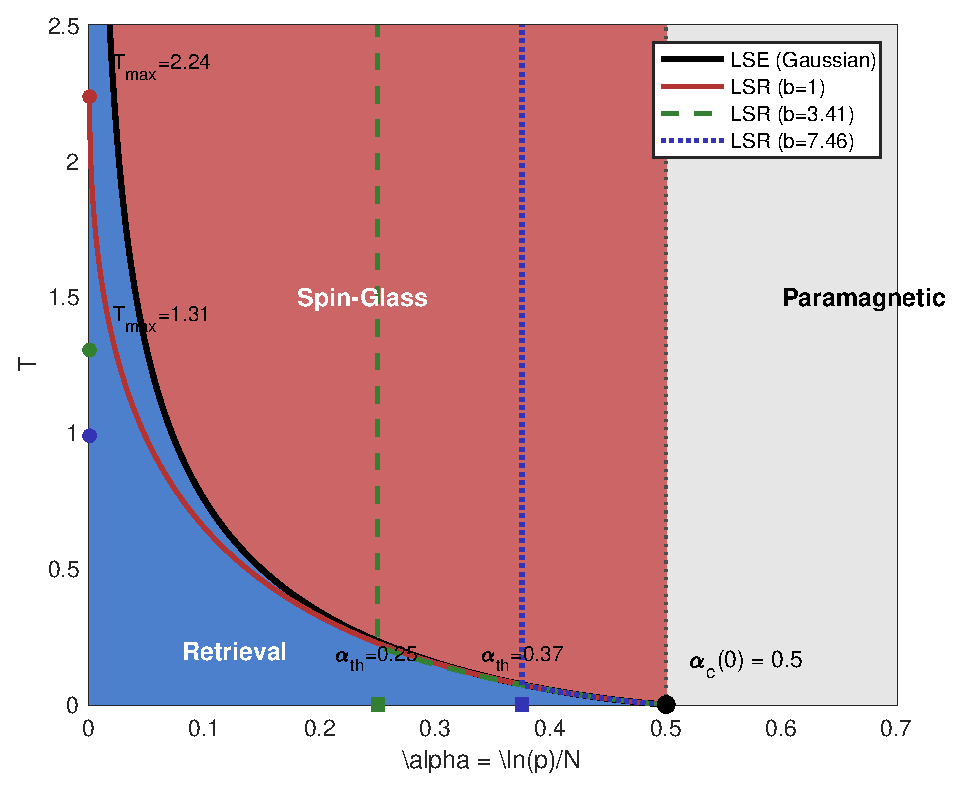
\includegraphics[width=\columnwidth]{fig_phase_diagram_3.eps}}
    \caption{Phase diagram for spherical DAM with exponential capacity $p = e^{\alpha N}$. The retrieval region (shaded) is bounded by the critical line $\alpha_c(T)$. LSE (solid black) permits retrieval at arbitrarily high temperatures, while LSR (dashed) exhibits a maximum temperature $T_{\max} \approx 2.23$. The boundary at $\alpha = 0.5$ separates spin-glass (SG) from paramagnetic (P) disordered phases.}
    \label{fig:phase_diagram}
  \end{center}
  \vskip -0.1in
\end{figure}

\begin{figure*}[t]
  \vskip 0.1in
  \begin{center}
    \centerline{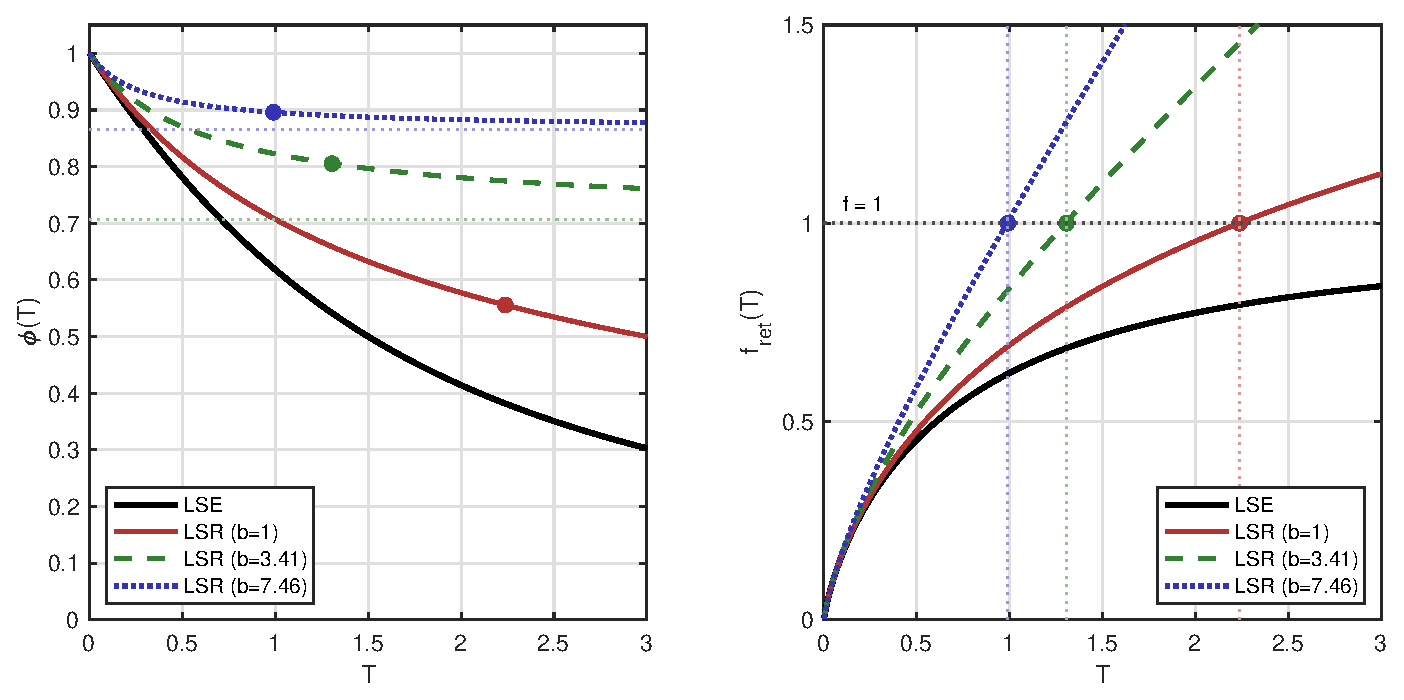
\includegraphics[width=\textwidth]{fig_equilibrium_3.eps}}
    \caption{Equilibrium properties vs temperature. \textit{Left:} Alignment $\phi(T)$ showing LSR maintains higher alignment due to its sharper well. \textit{Right:} Retrieval free energy $f_{\rm ret}(T)$ showing LSR grows faster, crossing the melting threshold $f = 1$ at finite $T_{\max}$.}
    \label{fig:equilibrium}
  \end{center}
  \vskip -0.1in
\end{figure*}

Figure~\ref{fig:equilibrium} compares the equilibrium alignment and free energy. The sharper LSR well maintains higher $\phi(T)$ at all temperatures, but this ``tightness'' incurs a larger entropy penalty, causing $f_{\rm ret}^{\rm LSR}$ to grow faster than $f_{\rm ret}^{\rm LSE}$.

\section{Conclusion}

We have derived the thermodynamic phase boundaries for Dense Associative Memory networks operating in the exponential capacity regime $p = e^{\alpha N}$. By separating the free energy into kernel-dependent energy and geometry-dependent entropy, we obtained analytic expressions for the critical line $\alpha_c(T)$ that delineates the retrieval phase from disordered (spin-glass or paramagnetic) phases.

Our central finding is a fundamental trade-off between energetic stability and entropic cost. The Epanechnikov (LSR) kernel creates deeper energy wells that maintain higher alignment $\phi(T)$ at finite temperature. However, this tighter confinement incurs a larger geometric entropy penalty: the system must pay an entropic cost proportional to $-\frac{1}{2}\ln(1-\phi^2)$ for maintaining high alignment in high-dimensional spherical geometry. This penalty grows faster for LSR than for LSE, causing the LSR retrieval free energy to exceed the melting threshold at a finite maximum temperature $T_{\max} \approx 2.23$.

The practical implications are twofold. First, kernel choice involves a robustness-capacity trade-off: LSE provides unlimited thermal robustness at the cost of shallower energy basins, while LSR offers sharper discrimination but finite temperature tolerance. Second, both kernels achieve the same zero-temperature capacity $\alpha_c(0) = 0.5$, confirming that exponential storage capacity is a geometric property of the spherical constraint rather than a kernel-specific feature.

These results extend classical spin-glass theory to modern attention-like memory architectures. Future directions include: (i) analyzing intermediate kernel families to map the full trade-off landscape, (ii) incorporating finite-size corrections for practical network sizes, and (iii) connecting the geometric entropy framework to the attention temperature in Transformer models.






%\section*{Software and Data}



% Acknowledgements should only appear in the accepted version.
%\section*{Acknowledgements}

%\textbf{Do not} include acknowledgements in the initial version of the paper
%submitted for blind review.

%If a paper is accepted, the final camera-ready version can (and usually should)
%include acknowledgements.  Such acknowledgements should be placed at the end of
%the section, in an unnumbered section that does not count towards the paper
%page limit. Typically, this will include thanks to reviewers who gave useful
%comments, to colleagues who contributed to the ideas, and to funding agencies
%and corporate sponsors that provided financial support.

\section*{Impact Statement}

This paper advances the theoretical understanding of high-capacity associative memory by deriving thermodynamic phase boundaries for continuous Dense Associative Memory networks on the $N$-sphere. The results are analytical and characterize when retrieval remains stable under noise (finite temperature) and exponential memory load, with potential relevance to attention-like mechanisms used in modern neural architectures. As a theoretical contribution, this work aims to clarify fundamental limits on memory robustness in high-dimensional systems. We do not introduce new datasets, user-facing systems, or deployment procedures, and our analysis does not involve personal data or human-subject experiments. Any broader impacts are therefore indirect: improved understanding of retrieval dynamics may inform the design of more reliable or efficient learning systems, while the same insights could be applied to optimize large-scale neural models, with societal implications similar to those associated with general advances in machine learning theory.



% In the unusual situation where you want a paper to appear in the
% references without citing it in the main text, use \nocite
\nocite{langley00}

\bibliography{dense_am}
\bibliographystyle{icml2026}

%%%%%%%%%%%%%%%%%%%%%%%%%%%%%%%%%%%%%%%%%%%%%%%%%%%%%%%%%%%%%%%%%%%%%%%%%%%%%%%
%%%%%%%%%%%%%%%%%%%%%%%%%%%%%%%%%%%%%%%%%%%%%%%%%%%%%%%%%%%%%%%%%%%%%%%%%%%%%%%
% APPENDIX
%%%%%%%%%%%%%%%%%%%%%%%%%%%%%%%%%%%%%%%%%%%%%%%%%%%%%%%%%%%%%%%%%%%%%%%%%%%%%%%
%%%%%%%%%%%%%%%%%%%%%%%%%%%%%%%%%%%%%%%%%%%%%%%%%%%%%%%%%%%%%%%%%%%%%%%%%%%%%%%
\newpage
\appendix
\onecolumn
\section{Derivation of the free energy density}

Let's write down the expression for $Z^n$ averaged over the the quenched disorder (locations of $\bm{\xi}^\mu$):
\begin{equation}
    \langle Z^n \rangle = \int \prod_{a=1}^n d\bm{x}_a \delta(|\bm{x}_a|^2 - N) \left\langle \exp\left(-\beta \sum_{a=1}^n H(\bm{x}^a, \bm{\xi}^\mu)\right) \right\rangle\,.
    \label{eq:Zn}
\end{equation}
Now let $\phi_a$ denote a replica sample of one alignment, e.g. corresponding to $\bm{\xi} = \bm{\xi}^\mu$, i.e. $\phi_a = \bm{x}_a \cdot \xi /N$ ($a=1\dots n$) and introduce the Overlap Matrix 
\begin{equation}
    q_{ab} = \frac{1}{N} \bm{x}_a \cdot \bm{x}_b\,.
\end{equation}
On the $N$-sphere, the diagonal elements are fixed: $q_{aa} =  \|\bm{x}_a\|^2/N = 1$. The off-diagonal elements $q_{ab}$ (for $a \neq b$) represent the Edwards-Anderson order parameter~\cite{ea75}, measuring how similar the configurations of two different replicas are.

We insert the identity 
\begin{equation}
1 = \int \prod_a \dd \phi_a \int \prod_{b<c} \dd q_{bc} \prod_a \delta\left(\phi_a - \bm{x}_a \cdot \bm{\xi}/N\right) \prod_{b<c} \delta\left(q_{bc} - \bm{x}_b \cdot \bm{x}_c/N\right)\,,
\end{equation}
where $\delta(\cdot)$ denotes the Dirac delta functions, into (\ref{eq:Zn}) and rearrange the order of integration:
\begin{multline}
\langle Z^n \rangle = \int \prod_a \dd \phi_a \int \prod_{b<c}  \dd q_{bc} \left\langle \int \prod_d \dd \bm{x}_d \delta(\|\bm{x}_d\|^2 - N) \prod_a \delta(\phi_a - \bm{x}_a \cdot \bm{\xi}/N) \right. \times \\
\left. \prod_{a<b} \delta(q_{bc} - \bm{x}_b \cdot \bm{x}_c/N) \exp\left(-\beta \sum_d H(\bm{x}_d, \bm{\xi}^\mu)\right) \right\rangle \,.
\end{multline}

For a Dense Associative Memory, the Hamiltonian $H$ is a function of the alignments. When the state is in the retrieval basin of $\bm{\xi}$, the density $p(\bm{x}, \bm{\xi}^\mu)$ (see Eq. \ref{eq:dens}) is dominated by the signal from that memory,
\begin{equation}
    p(\bm{x}, \bm{\xi}^\mu) \approx \exp\left[ - \frac{\beta_{\rm net}}{2} d^2(\bm{x}, \bm{\xi}) \right] \,.
    \label{eq:dens_red}    
\end{equation}
Thus, we can replace the microscopic $H(\bm{x}_a, \bm{\xi}^\mu)$ with a macroscopic potential that depends only on the alignment variable $\phi_a$:
\begin{equation}
    H(\bm{x}^a, \bm{\xi}^\mu) \to \mathcal{U}(\phi_a) = -\frac{1}{\beta_{\rm net}} \ln \left[  \exp\left( -\frac{N(1 - \phi_a)}{\sigma^2} \right) \right] = N(1-\phi_a)
\end{equation}
for LSE kernel. Since $\mathcal{U}(\phi^a)$ is no longer a function of the integration variable $\bm{x}^a$, we factor it out of the microscopic integral:
\begin{equation}
    \langle Z^n \rangle = \int \prod_a \dd \phi_a \int \prod_{b<c}  \dd q_{bc} \exp\left(-\beta \sum_a \mathcal{U}(\phi^a)\right)  \Omega(\phi_a, q_{bc})
\end{equation}


The remaining term, $\Omega(\phi_a, q_{bc})$, is the average over the memories of the volume of the configuration space that satisfies the macroscopic constraints:
\begin{equation}
\Omega(\phi_a, q_{bc}) = \left\langle \int \prod_d \dd \bm{x}_d \prod_d \delta(\|\bm{x}_d\|^2 - N) \prod_a \delta(\phi_a - \bm{x}_a \cdot \bm{\xi}/N) \prod_{b<c} \delta(q_{bc} - \bm{x}_b \cdot \bm{x}_c/N) \right\rangle\,.
\end{equation}
This is a purely geometric quantity. It counts how many ways we can arrange $n$ vectors on an $N$-sphere such that their lengths are $\sqrt{N}$, their projections on the memory vector are fixed by $\phi_a$, and their mutual angles are fixed by $q_{bc}$.

In the limit $N \to \infty$, the configuration volume $\Omega$ scales exponentially with $N$. We define the geometric entropy density $s$ as:
$$s(\phi_a, q_{bc}) = \lim_{N \to \infty} \frac{1}{N} \ln \Omega(\phi_a, q_{bc})$$
Similarly, the internal energy scales linearly with $N$: $u(\phi) = \mathcal{U}(\phi)/N$. Substituting these into the expression:
\begin{equation}
    \langle Z^n \rangle \approx \int \prod_a \dd \phi_a \int \prod_{b<c}  \dd q_{bc} \exp\left( N \left[ -\beta \sum_a u(\phi_a) + s(\phi_a, q_{bc}) \right] \right)
\end{equation}

To solve the integral, we assume the Replica Symmetric ansatz~\cite{amit1987statistical}: all replicas are identical, i.e. $\phi_a = \phi$ for all $a$, and $q_{ab} = q$ for all $a \neq b$. Under this assumption, the high-dimensional integral over the $n$ alignment variables and $n(n-1)/2$ overlap variables reduces to a two-dimensional integral over the order parameters $\phi$ and $q$. The replicated partition function $\langle Z^n \rangle$ is then given by:
\begin{equation}
\langle Z^n \rangle \approx \int \dd \phi \int \dd q \exp \left( N n \left[ -\beta u(\phi) + s(\phi, q) \right] \right)
\end{equation}

The entropy density arises from the volume of microstates that satisfy the alignment $\phi$ and the overlap $q$~\cite{ea75}. For continuous variables on an $N$-sphere, the entropy can be obtained analytically~\citep[see][for details]{gardner1988space}:
\begin{equation}
    s(\phi, q) = \frac{1}{2} \left[ \ln(1-q) + \frac{q - \phi^2}{1-q} \right] + \text{const.}
\end{equation}

In the thermodynamic limit ($N \to \infty$), the integral is dominated by the specific values of $\phi=\phi_*$ and $q=q_*$ that maximize the exponent (the saddle point):
\begin{equation}
    \beta \frac{\partial u}{\partial \phi} + \frac{\phi}{1-q} = 0\,,\qquad 
    \frac{1}{1-q} - \frac{1-\phi^2}{(1-q)^2} = 0\,.
\end{equation}
The second equation implies $q_* = \phi_*^2$, meaning that in the retrieval phase, the ``tightness'' of the thermal cloud $q_*$ is entirely determined by its distance from the origin (alignment $\phi_*$). In the equilibrium values $(\phi_*, q_*)$, the exponent is stationary. Thus we obtain:
\begin{equation}
    \langle Z^n \rangle \approx \exp\left( N n [-\beta u(\phi) + s(\phi, q)] \right)
\end{equation}
Applying the limit (\ref{eq:limit}) leads to the final result:
\begin{equation}
    \langle f \rangle = -\frac{1}{N\beta} \langle \ln Z \rangle 
    \approx  u(\phi) - T s(\phi, q)\,.
\end{equation}

\section{Derivation of the Internal Energy Density for the LSR Kernel}

To determine the internal energy density $u(\phi)$ for the Log-Sum-ReLU (LSR) Hamiltonian, one should account for the scaling of Euclidean distances and kernel parameters in the high-dimensional limit ($N \to \infty$). The internal energy of the network using the Epanechnikov kernel is defined by the Hamiltonian (\ref{eq:H_lsr}), with $d^2(\mathbf{x}, \boldsymbol{\xi}^\mu) = 2N(1 - \phi^\mu)$. 
For fixed $\sigma^2$, in the limit of $N \to \infty$, the retrieval basin of a pattern shrinks to zero. To maintain a retrieval basin that spans a macroscopic range of alignments $\phi \in [0, 1]$, the kernel width $\sigma^2$ must scale linearly with $N$. So, we define the normalized width $\hat{\sigma}^2$ as $\sigma^2 = N \hat{\sigma}^2$, and $\hat\beta_{\rm net} = N \beta_{\rm net}$. The latter scaling ensures  that the LSR internal energy density $u = H/N$ is comparable to the LSE case and that the energy basins have identical slopes at the point of perfect retrieval.

Assuming the system is in the retrieval basin of pattern $\bm{\xi}$, the sum is reduced to a single term. Substituting the scaled parameters into the Hamiltonian:
\begin{equation}
H_{\text{LSR}}(\phi) \approx -N \hat{\sigma}^2 \ln \left( 1 - \frac{2N(1-\phi)}{2N\hat{\sigma}^2} \right).
\end{equation}
Dividing by $N$, we obtain the macroscopic internal energy density used in the free energy evaluation:
\begin{equation}
u_{\text{LSR}}(\phi) = -\hat{\sigma}^2 \ln \left( 1 - \frac{1-\phi}{\hat{\sigma}^2} \right) = -\frac{1}{\hat\beta_{\rm net}} \ln \left( 1 - \hat\beta_{\rm net}(1-\phi) \right).
\end{equation}
Near $\phi=1$, the Taylor expansion yields $u_{\text{LSR}}(\phi) \approx (1-\phi) + (1-\phi)^2 /(2\hat{\sigma}^2) + \dots$, confirming that LSR behaves like a quadratic correction to the linear LSE basin. The logarithmic form ensures that the energy penalty grows significantly as the state deviates from the pattern, leading to the sharper retrieval dynamics observed in LSR.

%%%%%%%%%%%%%%%%%%%%%%%%%%%%%%%%%%%%%%%%%%%%%%%%%%%%%%%%%%%%%%%%%%%%%%%%%%%%%%%
%%%%%%%%%%%%%%%%%%%%%%%%%%%%%%%%%%%%%%%%%%%%%%%%%%%%%%%%%%%%%%%%%%%%%%%%%%%%%%%

\end{document}

% This document was modified from the file originally made available by
% Pat Langley and Andrea Danyluk for ICML-2K. This version was created
% by Iain Murray in 2018, and modified by Alexandre Bouchard in
% 2019 and 2021 and by Csaba Szepesvari, Gang Niu and Sivan Sabato in 2022.
% Modified again in 2023 and 2024 by Sivan Sabato and Jonathan Scarlett.
% Previous contributors include Dan Roy, Lise Getoor and Tobias
% Scheffer, which was slightly modified from the 2010 version by
% Thorsten Joachims & Johannes Fuernkranz, slightly modified from the
% 2009 version by Kiri Wagstaff and Sam Roweis's 2008 version, which is
% slightly modified from Prasad Tadepalli's 2007 version which is a
% lightly changed version of the previous year's version by Andrew
% Moore, which was in turn edited from those of Kristian Kersting and
% Codrina Lauth. Alex Smola contributed to the algorithmic style files.




